% XCircuit output "linear_quantizer_model.tex" for LaTeX input from linear_quantizer_model.ps
\def\putbox#1#2#3{\makebox[0in][l]{\makebox[#1][l]{}\raisebox{\baselineskip}[0in][0in]{\raisebox{#2}[0in][0in]{#3}}}}
\def\rightbox#1{\makebox[0in][r]{#1}}
\def\centbox#1{\makebox[0in]{#1}}
\def\topbox#1{\raisebox{-\baselineskip}[0in][0in]{#1}}
\def\midbox#1{\raisebox{-0.5\baselineskip}[0in][0in]{#1}}
\begin{flushleft}
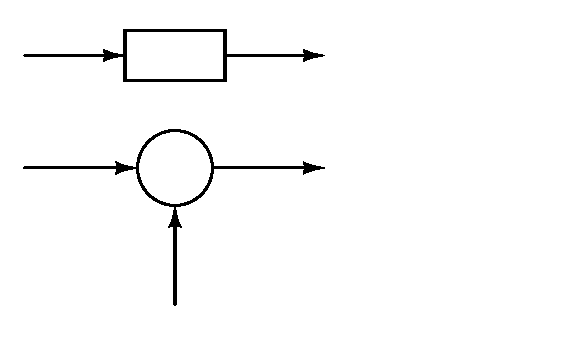
\epsfig{file=linear_quantizer_model.ps}\\
% translate x=416 y=409 scale 0.38
\putbox{0.76in}{1.89in}{\midbox{Quantizer}}%
\putbox{0.06in}{2.02in}{\midbox{$x(n)$}}%
\putbox{1.72in}{2.02in}{\midbox{$\hat{x}(n)=\mathcal{Q}\bigl[x(n)\bigr]$}}%
\putbox{1.06in}{1.14in}{\centbox{\midbox{$\displaystyle\sum$}}}%
\putbox{0.06in}{1.27in}{\midbox{$x(n)$}}%
\putbox{0.93in}{0.10in}{\midbox{$e(n)$}}%
\putbox{1.72in}{1.27in}{\midbox{$\hat{x}(n)=x(n)+e(n)$}}%
\end{flushleft}
